\section{Kong}
Kong Gateway es una pasarela de API nativa en la nube ligera, rápida 
y flexible y un proxy inverso que le permite gestionar, configurar y 
dirigir las solicitudes a sus API. \cite{kong-api-gateway}

\subsection{Arquitectura desentralizada}
Kong está construido sobre una arquitectura descentralizada, 
lo que permite desplegar y gestionar API en múltiples entornos, 
ya sea en la nube, on-premise o en una configuración híbrida. 
Esto facilita la escalabilidad y la resistencia del sistema.


\subsubsection{Automatización de Flujos de Trabajo y GitOps Modernos}
Kong se integra con prácticas modernas como GitOps, que permiten la automatización de 
flujos de trabajo a través del control de versiones de la infraestructura y las configuraciones. 
Esto asegura que las implementaciones sean consistentes y rastreables, lo cual es esencial en entornos descentralizados.

\subsubsection{Ecosistema de Desarrolladores de API}
Al descentralizar las aplicaciones y servicios, Kong Gateway facilita la creación 
de un ecosistema vibrante para los desarrolladores de API. Los equipos pueden 
trabajar de manera independiente en diferentes servicios, lo que acelera el 
desarrollo y la implementación de nuevas funcionalidades.

\subsubsection{Identificación Proactiva de Anomalías y Amenazas}
La arquitectura descentralizada, junto con las capacidades avanzadas de Kong, 
permite una identificación proactiva de anomalías y amenazas 
relacionadas con las API. Esto es esencial para mantener 
la seguridad y el rendimiento en un entorno distribuido.

\subsubsection{Gobernanza y Seguridad de APIs}
Kong proporciona herramientas para la seguridad y la gobernanza de las API, 
mejorando la visibilidad y el control en toda la organización. 
Esto es crucial en arquitecturas descentralizadas, donde es necesario mantener un 
alto nivel de seguridad y cumplimiento normativo a través de múltiples servicios y entornos.


\subsection{Plugins Personalizables}
Kong ofrece una amplia variedad de plugins que pueden ser utilizados para añadir 
funcionalidades como autenticación, limitación de tasa, caché, entre otros. Además, 
permite a los usuarios crear sus propios plugins personalizados para satisfacer necesidades específicas.

\subsection{Seguridad}
Kong proporciona diversas herramientas para asegurar las API, incluyendo autenticación 
JWT (JSON Web Token), OAuth2, mTLS (mutual TLS), y cifrado de tráfico. 
La capacidad de implementar políticas de seguridad a través de sus plugins 
hace que Kong sea una opción confiable para la protección de API.


\subsection{Monitoreo y Observabilidad}
Kong ofrece integración con herramientas de monitoreo como Prometheus, Grafana, y 
otras soluciones de observabilidad para rastrear el rendimiento de las API, errores,
y métricas clave. Esto permite una gestión proactiva y la resolución rápida de problemas.

% TODO: Ayuda acá 
\subsection{Konnect Advanced Analytics}
Konnect Advanced Analytics es una plataforma en tiempo real que ofrece análisis detallados 
de APIs para optimizar estrategias y mejorar la eficiencia operativa. Disponible como 
servicio premium en Konnect. \cite{konnect-advanced-analytics}

\begin{itemize}
  \item \textbf{Visibilidad centralizada}: Proporciona una visión integral y centralizada de todo el panorama de tus API para todas las APIs, servicios y planos de datos.
  \item \textbf{Analítica contextual de API}: Konnect Advanced Analytics ofrece información sobre cada solicitud de API, incluyendo las rutas específicas, los consumidores involucrados, y los servicios accedidos.
  \item \textbf{Insights de datos democratizados}: Konnect empodera tanto a los equipos de negocio como a los de plataforma para generar informes para cualquier servicio, ruta, o consumidor, basados en sus requisitos específicos.
  \item \textbf{El tiempo más rápido para obtener insights}: Proporciona a los equipos de aplicaciones y plataformas métricas críticas de API para cada servicio en menos de un segundo, reduciendo así el tiempo de resolución.
  \item \textbf{Reducción del costo de propiedad}: Advanced Analytics es una solución de analítica llave en mano que elimina la necesidad de construir, mantener o integrarse con productos de terceros.
\end{itemize}

\subsection*{Servicios y Rutas}

Kong Gateway utiliza un modelo de objetos para definir políticas de gestión de tráfico. 
Los objetos clave, como servicios y rutas, se configuran de manera coordinada para establecer 
el flujo de solicitudes y respuestas en el sistema. Las solicitudes se enrutan a los servicios 
a través de las rutas definidas, mientras que las respuestas siguen el camino inverso, tal como se describe en 
la siguiente imagén. \cite{kong-services-routes}

\begin{figure}[h!]
  \centering
  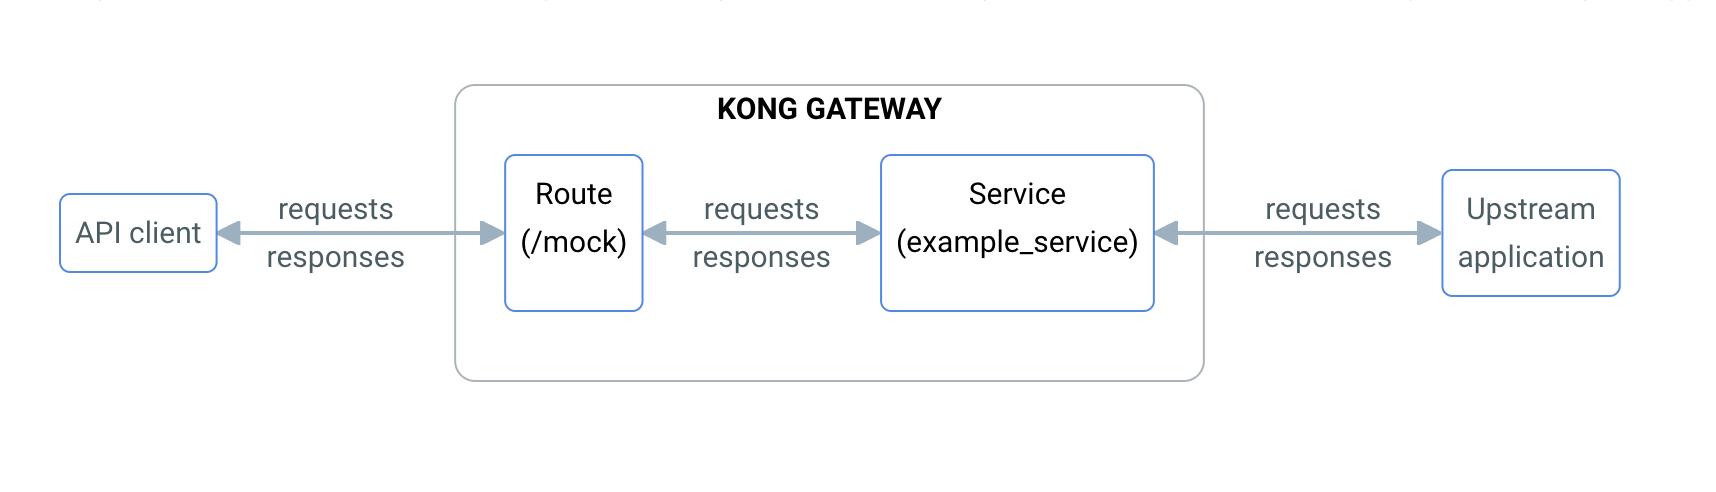
\includegraphics[width=\columnwidth]{images/kong-gateway.png}
  \caption{Kong Gateway - Rutas y servicios}
  \label{fig:kong_gateway_rutas_servicios}
\end{figure}

\subsubsection*{Servicio}
En Kong Gateway, un servicio es una abstracción de una aplicación upstream existente. 
Los servicios pueden almacenar colecciones de objetos como configuraciones de plugins y políticas, y pueden asociarse con rutas.

Al definir un servicio, se proporciona un nombre y la información de conexión a 
la aplicación upstream. Estos detalles de conexión pueden especificarse en un solo 
campo URL o separadamente en los campos de protocolo, host, puerto y ruta.

Los servicios tienen una relación de uno a muchos con las aplicaciones upstream, 
lo que permite crear comportamientos avanzados de gestión de tráfico.

\subsubsection*{Ruta}

Una ruta es un camino hacia un recurso dentro de una aplicación upstream. 
Las rutas se añaden a los servicios para permitir el acceso a la aplicación subyacente. 
En Kong Gateway, las rutas suelen mapearse a endpoints expuestos a través de la aplicación Kong Gateway. 
Además, las rutas pueden definir reglas que relacionan solicitudes con servicios asociados, 
lo que permite que una ruta pueda referenciar múltiples endpoints. Una ruta básica debe tener un nombre, 
una o varias rutas, y referenciar a un servicio existente.

% Fuentes: 
% https://docs.konghq.com/gateway/latest/
% https://docs.konghq.com/konnect/analytics/
% https://docs.konghq.com/gateway/latest/get-started/services-and-routes/

% \begin{thebibliography}{9}
% \bibitem{kong} Kong Gateway: Servicios y Rutas. \textit{KongHQ Documentation}. Disponible en: \url{https://docs.konghq.com/gateway/latest/get-started/services-and-routes/}
% \end{thebibliography}